\section{Background}
\label{sec:problem}

LN allows two counterparties to agree on an off-chain allocation of arbitrary amount of funds. It ensures the off-chain security with the RSMC and HTLC mechanisms.

\begin{figure}[t]
\centering
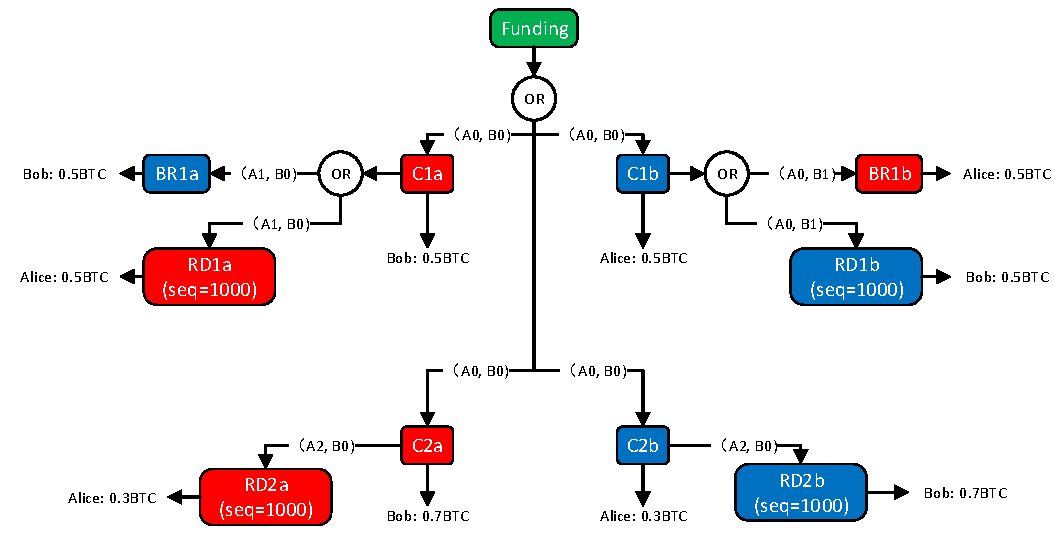
\includegraphics[width=3.5in]{figs/rsmc_old.pdf}
\vspace{-12pt}
\caption{RSMC (Revocable Sequence Maturity Contract)}
\label{fig:RSMC}
\end{figure}


Figure~\ref{fig:RSMC} reviews the RSMC mechanism. RSMC generates a pair of Commitment Transactions, each of which is held by one's counterparty. By broadcasting the Commitment Transaction, a counterparty has the ability to close the channel by spending the Funding Transaction. Accordingly, funds within channel are returned to both counterparties based on their latest agreement. To prevent old Commitment Transaction from being broadcast, RSMC places a LockTime on the funds of the counterparty who broadcasts. At the same time, it also enforces the exchange of private keys between two counterparties for old Commitment Transactions. If either party discovers that an old Commitment Transaction (e.g., C1a in Figure~\ref{fig:RSMC}) is broadcast, he/she can broadcast a penalty transaction (BR1a) with previously exchanged private keys to acquire all funds in the channel. Ensured by this mechanism, no one has the incentive to broadcast old Commitment Transactions.

\begin{figure}[t]
\centering
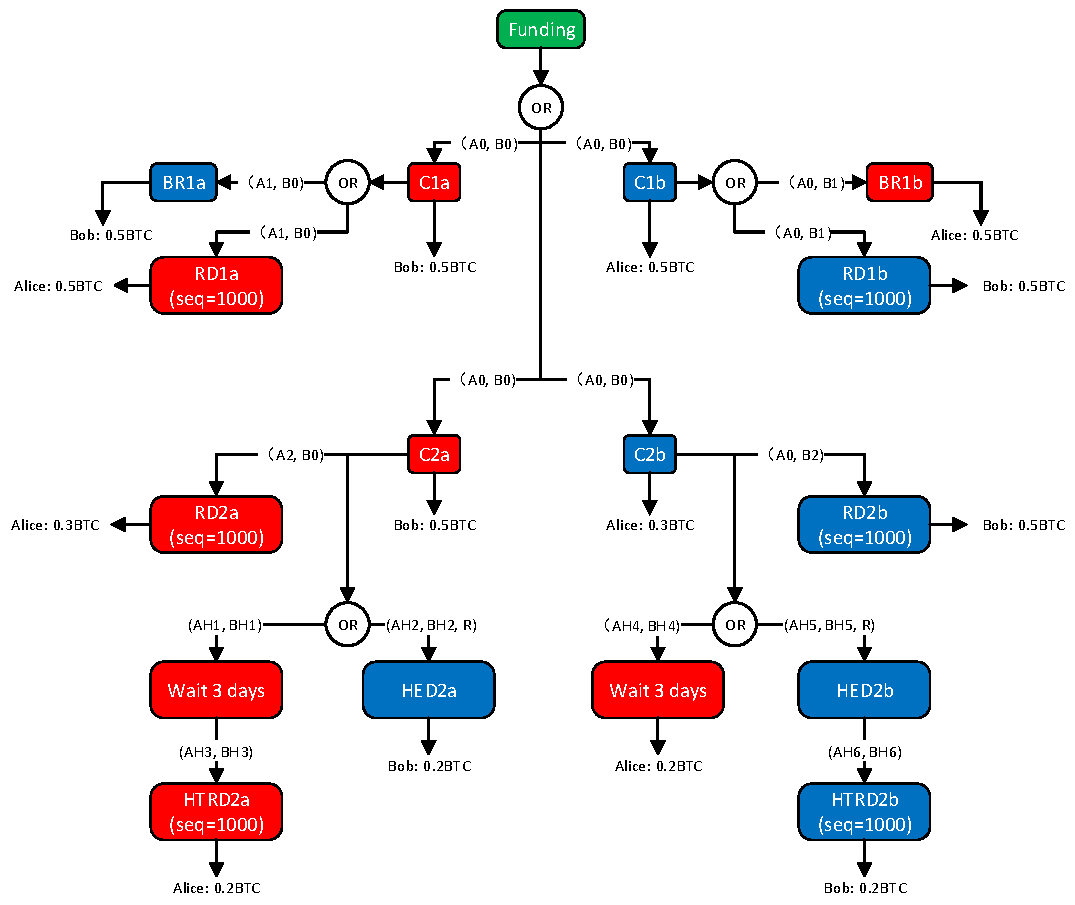
\includegraphics[width=3.5in]{figs/htlc_old.pdf}
\vspace{-12pt}
\caption{HTLC (Hashed Timelock Contract)}
\label{fig:htlc}
\end{figure}


The HTLC mechanism utilizes hash functions, ensured by transactional "locking" between two counterparties, to construct a secure network of channels across multiple destinations between the starting and ending participants\cite{poon2015bitcoin}. Specifically, if the receiver can produce a pre-image $R$ to fulfill a known pre-defined image $H(R)$, the sender pays the receiver. Figure~\ref{fig:htlc} shows the detailed protocol of HTLC, in combination with RSMC to forbid the broadcast of old agreements.


The major limitation of RSMC and HTLC is that funds in the channel cannot be dynamically adjusted unless both participants close and then reopen the channel. Once a channel is built, the total funds in a channel remains fixed. Existing design makes it impossible to deposit new funds into the channel or partially withdraw funds from the channel. Furthermore, the off-chain channel has different capacities in both directions. The capacities continue to change as funds are being transferred between participants, which results in the {\em channel dry-up} problem, meaning funds for that particular direction is exhausted. For instance, assuming one participant is a buyer and the other is a seller, the funds always goes from the buyer to the seller, causing a dry-up in this channel direction. In this case, both participants have to close the channel and recreate a new one. Closing and reopening channels are require to be broadcast, which give rise to extra costs and time delay.


Existing approaches solve the channel dry-up problem by rebalancing funds across multiple channels \cite{Khalil2017}. However, achieving a rebalance requires identification of a loop in the LN graph \cite{Khalil2017}. For example, when the unidirectional channel from A to B dries up, A can find a third-party participant C and transfer some funds to C. Then C transfers the same funds to B (consuming transaction fees). Finally, B transfers the funds back to A, which rebalances the channel between A and B.  This routing-based rebalance requires specific network topology since it is highly probable that no valid loop exists. In a case where a participant is a customer, he/she usually spends his/her channel funds instead of receiving payment from others. Therefore, it is very likely that his/her channels dry up quickly and fails to be rebalanced.
